\subsection{Approach, data and pre-processing}
\label{sec:overview}
This section describes the external data sources we used as well as our pre-processing steps.

%\subsubsection{The RCC Corpus}
%\label{subsec:rcc-corpus}
%For the first phase, the data provided by the organizers consisted of 5,000 publications. Additionally, a development fold of 100 plain text publications, their metadata, a list of datasets of interest (including all datasets that were explicitly referenced in the curated corpus) were given. The list of datasets should not be considered complete as  there could be additional datasets mentioned in these publications. 
%The organizers also provided examples of social science research methods and fields vocabularies in term of SAGE Publications research field and method vocabularies. 
%In the second phase of the competition, an additional set of 5,000 publications from the social sciences has been provided.

%TODO include subsubsection on "Approach overview and initial evaluation feedback" where we can include the overview of the modules and more details on the first stage evaluation (I've been cutting these parts a lot in the introduction to keep it more general)

\subsubsection{Approach overview and initial evaluation feedback}
\label{sec:approach_feedback}




%\subsection{Task Definition of the RCC}
%In both competition phases the task was to submit a software package which is able to process PDF (respectively extracted raw text) on the Servers of the organizers.
%The software have to be able to extract dataset mentions, research methods and research fields from the given publication. More about the type of scientific publications can be found in Section~\ref{subsec:rcc-corpus}.
%In the first phase additional the software has to be able to link dataset mentions to a given set of around 10,000 dataset descriptions originate from ICPSR\footnote{\url{https://www.icpsr.umich.edu/icpsrweb/ICPSR/}} research data index.


%\subsubsection{Non-technical overview}

%\begin{itemize}
%    \item Usage of external data
%    \item Supervised machine learning Approaches
%    \item Problem of Training data: weak supervision
%\end{itemize}


% Literature Review


The central tasks in the RCC are the extraction of dataset mentions from text. 
Even so, we considered the discovery of research methods and research fields important.
To this end, we decided to follow a module-based approach. Users could choose to use each specific module solely or as parts of a data processing pipeline.
Figure~\ref{figure:pipeline} shows an overview of modules developed and their dependencies.
Here, the upper three modules (which are in gray) describe the pre-processing steps (cf. Section~\ref{sec:prepro}).
The lower four modules (blue) are used to generate the output in a predefined format as specified by the competition.


\begin{figure}[t]
    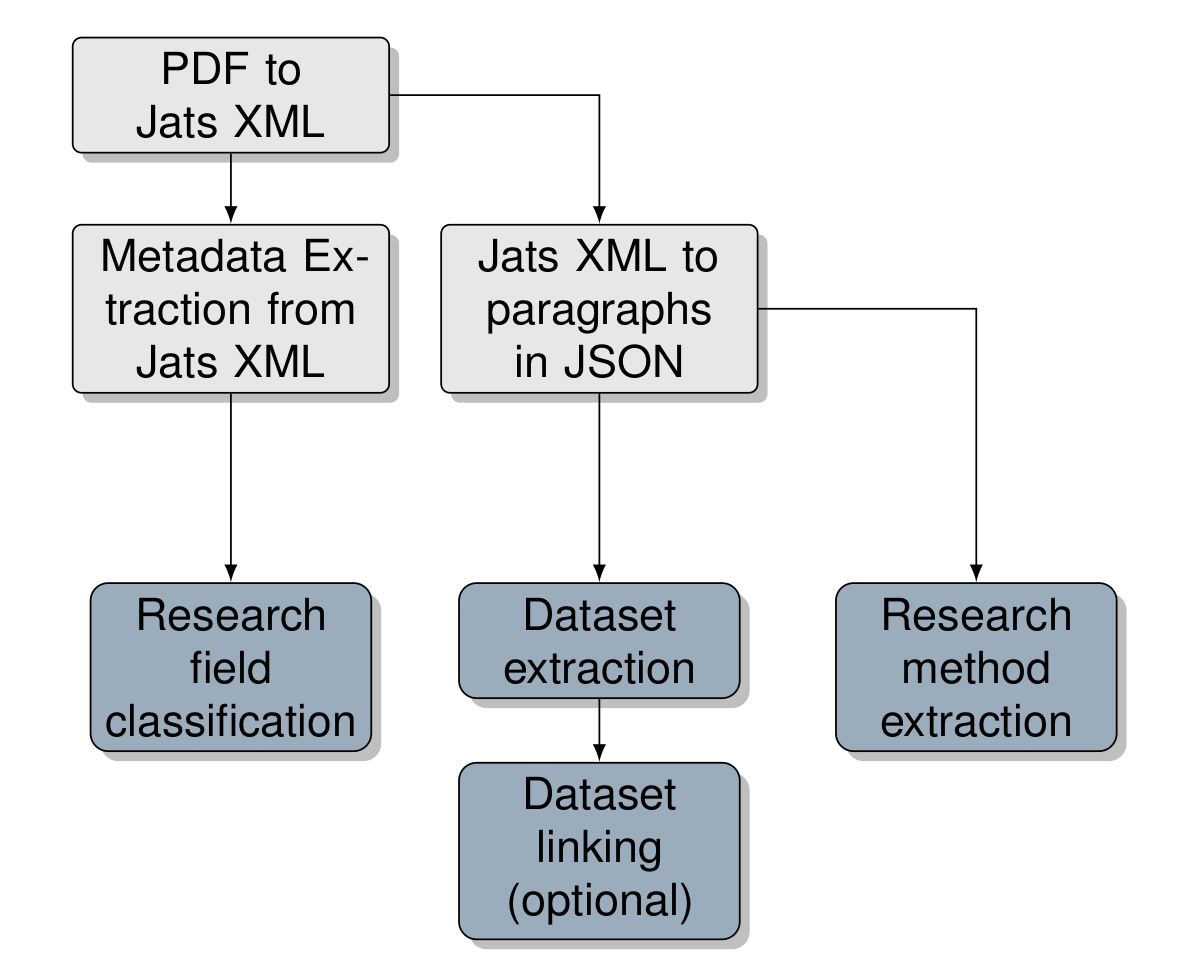
\includegraphics[width=0.47\textwidth]{figures/information-flow.png}
    %% Graphic from tex
    %\resizebox{!}{7cm}{\tikzset{
  basic/.style  = {draw, text width=2cm, drop shadow, font=\sffamily, rectangle},
  root/.style   = {basic, rounded corners=2pt, thin, align=center,
                   fill=color1!30},
  level empty/.style={},
  level 1/.style={sibling distance=2mm},
  level 2/.style = {basic, rounded corners=4pt, thin, align=center, fill=color1!60},
  level 3/.style = {basic, rounded corners=2pt, thin,
                    align=center, fill=color2!10, text width=6.5em}
}


\begin{tikzpicture}[
  node distance=1.7cm and 1.7cm,
  edge from parent/.style={->,draw},
  >=latex
  ]

% root of the the initial tree, level 1
%\node[root] {RCC-05 Pipeline Components}
% The first level, as children of the initial tree
%  child {node[level 2] (c1) {Preprocessing}}
%  child {node[level 2] (c2) {Dataset Linking}}
%  child {node[level 2] (c3) {Research Method Extraction}}
%  child {node[level 2] (c4) {Research Field Classification}};

% The second level, relatively positioned nodes
\begin{scope}[every node/.style={level 3}]
    \node [] (c11) {PDF to Jats XML};
    \node [below of = c11] (c12) {Metadata Extraction from Jats XML};
    \node [right = 0.4cm of c12] (c13) {Jats XML to paragraphs in JSON};
\end{scope}

\node [level 2, below = 1.5cm of c13, xshift=0pt] (c21) {Dataset extraction};
\node [level 2, below =  0.5cm of c21] (c22) {Dataset linking (optional)};
\node [level 2, below = 1.5cm of c13, xshift=3cm]  (c31) {Research method extraction};
\node [level 2, below = 1.5cm of c12, xshift=0pt] (c41) {Research field classification};

\node [level empty, below = 2.7cm of c21] (c51){};
 



% lines from each level 1 node to every one of its "children"
%\foreach \value in {1,...,3}
%  \draw[->] (c1.195) |- (c1\value.west);
%\draw[->] (c1.south) -| (c11.north);
\draw[->] (c11.south) -| (c12.north);
\draw[->] (c11.east)  -- +(1,0) -| (c13.north);

\draw[->] (c13.south) -| (c21.north);
\draw[->] (c21.south) -| (c22.north);

\draw[->] (c13.east) -- +(1.7,0) -| (c31.north);

\draw[->] (c12.south) -| (c41.north);

%\foreach \value in {1,...,1}
%  \draw[->] (c3.195) |- (c3\value.west);
\end{tikzpicture}

\begin{comment}
    Old Pipeline (4 Elements)
    \node[level 2] (c1) {(1) Preprocessing};
    \node[level 2, right= 3cm of c1] (c2) {(2) Dataset Linking};
    \node[level 2, right= of c2] (c3) {(3) Research Method Extraction};
    \node[level 2, right= of c3] (c4) {(4) Research Field Classification};
    \draw[->] (c1) |- (c2);
    \draw[->] (c1.30) -- +(0,0.7) -| (c3.north);
    \draw[->] (c1.150) -- +(0,1.3) -| (c4.north);

\end{comment}
}
    \caption{An overview of the individual software modules described in this document and their dependencies. 1- Gray: Our pre-processing pipeline. 2- Blue: three main tasks of the RCC.}
    \label{figure:pipeline}
\end{figure}

%TODO I'd suggest to use the same wording in the figure as in the following section headings, e.g. "Resarch field classification" etc. Also, I would not use color-coding (always ambiguous on b/w printing).

The pre-processing step consists of extracting metadata and raw text from PDF documents.
The output of this step is then used by the software modules responsible for tackling the individual sub-tasks.
These sub-tasks are to discover research datasets (cf. Section~\ref{sec:dataset-extraction}), methods (cf. Section~\ref{sec:research_method_extraction}) and fields (cf. Section~\ref{sec:field_classification}).
First, a Named Entity Recognition module is used to find dataset mentions.
This module used a supervised approach trained on a weakly labled corpus.
%The creation of the used training corpus and the model are described in Section~\ref{sec:dataset-extraction}.
In the next step, we combine all recognized mentions for each publication and compare these mentions to the metadata from the list of datasets given by the competition. %`data_sets.json`.
For this linking step the mentions and year information located in the same sentence are used.
The corresponding sentence and extracted information are saved for debugging and potential usage in future pipeline components.
%After retrieving the best matching results, theses are returned in the target format specified by the RCC-competition.
The task of identifying research methods is solved unsing a Named Entity Recognition and Linking module with incorporated word embeddings and lexical resources. 
For identifying research fields, we trained a classifier on openly available abstracts and metadata from the domain of social sciences crawled from the Social Science Open Access Repository\footnote{\url{https://www.ssoar.info}} (SSOAR).
%We used the OAI-API for this and the crawler is delivered in the module.
We tried different classifiers and selected the best performing one, a classifier based on fasttext\footnote{\url{https://fasttext.cc/}}, i.e. a neural net based approach with a high performance\cite{joulin2017bag}.



After the first phase, each team received feedback from the organizers of the RCC.
The feedback is two folds, a quantitative and qualitative evaluation.
Unfortunately, the quantitative assessment showed our algorithm for dataset mention retrieval did not perform well regarding precision and recall metrics.
In contrast to this, our approach has been found convincing regarding the quality of results.
The qualitative feedback is based on a random sample of ten documents given to four judges.
The judges were asked to manually extract dataset mentions.
After this the overlap between their dataset extractions and the output of our algorithm was calculated.
Other factors that judges took into consideration are specificity, uniqueness, and multiple occurrences of dataset mentions.
As for the extraction of research methods and fields, no ground truth has been provided; these tasks were evaluated against the judges' expert knowledge.
Similarly to the extraction of dataset mentions, specificity and uniqueness have been considered for these two tasks.
The feedback our team received was overall positive.
% ..acknowledged the fact that no ground truth has been provided and our efforts regarding the extraction of research methods and fields.
%Feedback by RCC
%Section~\ref{} gives detailed overview of data provided by the RCC and additional data sources used in our approach.

\subsubsection{External data sources}
\label{sec:external_data_sources}
For developing our algorithms, we utilized two external data sources.
For the discovery of research methods and fields, we resort to data from the Social Science Open Access Repository\footnote{\url{https://www.gesis.org/ssoar/home}} (SSOAR). 
GESIS – Leibniz Institute for the Social Sciences maintains  SSOAR by collecting and archiving literature of relevance to the social sciences. 

In SSOAR, full texts are indexed using controlled social science vocabulary (Thesaurus\footnote{\url{https://www.gesis.org/en/services/research/tools/thesaurus-for-the-social-sciences}}, Classification\footnote{\url{https://www.gesis.org/angebot/recherchieren/tools-zur-recherche/klassifikation-sozialwissenschaften} (in German)}) and are assigned rich metadata. SSOAR offers documents in various languages. The corpus of English language publications that can be used for purposes of the competition consists of a total of 13,175 documents. All SSOAR documents can be accessed through the OAI-PMH\footnote{{\url{http://www.openarchives.org}}} interface. 

Another external source we have used to discover research methods is the ACL Anthology Reference Corpus~\cite{bird2008acl}. ACL ARC is a corpus of scholarly publications about computational linguistics.  
The corpus consists of a total of 22,878 articles.

%SSOAR contains 
%\subsubsection{SSOAR}
%\label{subsubsec:ssoar-dataset}
%For example, 22,453 records with English abstracts in SSOAR also contain information about the classification of social sciences documents - 156 different labels of the classification.
%For items with English title and classoz classification, the numbers are different. SSOAR includes 15,522 items with English titles and cover 154 classoz classification labels.
%Classification Schemes used in the anntotations of SSOAR publications.
%\begin{enumerate}
%    \item Thesaurus Social Science (thesoz)
%    \item classification of the social sciences %(classoz)\footnote{\url{https://www.gesis.org/angebot/recherchieren/tools-zur-recherche/klassifikation-sozialwissenschaften} (in German)}
%    \item ddc classification (ddc)
%\end{enumerate}

%\subsubsection{ACL}
%ACL 

%\dd{table of external data/sources?SSOAR metedata including abstracts and classifications(thesoz/ classsoz)}

\subsubsection{Pre-processing}
\label{sec:prepro}
Although the organizers of the RCC offered plain texts for the publication, we decided to build our own pre-processing pipeline.
The extraction of text from PDF files is still an error prone process. To handle de-hyphenation and paragraph segmentation during extraction time and benefit from automatic metadata extraction (i.e. title, author, abstracts and references) we decided to use a third party extraction tool.
The Cermine Extraction Tool\footnote{\url{https://github.com/CeON/CERMINE}}\cite{tkaczyk2015cermine} transforms the files into XML documents using the Journal Article Tag Suite\footnote{\url{https://jats.nlm.nih.gov}}(Jats).
%The main benefit of using this tool is the structured metadata output, including better disambiguation of sections and paragraphs in the publications.
For the competition we identified two interesting elements of the Jats XML format, i.e., $<$front$>$ and $<$body$>$. The $<$front$>$ element contains the metadata of the publication, whereas the $<$body$>$ contains the main textual and graphic content of the publication.
%A benefit of Cermine is that the de-hyphenation and segmentation of paragraphs are carried out out of the box.
As a last step of the pre-processing, we removed all linebreaks from the publication.
The output of this step is a list of metadata fields and values, as shown in Table~\ref{tab:example-paragraph} for each publication paragraph.

\begin{table}[h]
    \centering
     \caption{Example preprocessing output for a paragraph in a given publication.}
    \begin{tabular}{ll}
        \toprule
        {}                  &                            Example Text Field Data \\
        \midrule
        publication\_id     &                                              12744 \\
        label               &                                    paragraph\_text \\
        text                &                     A careful reading of text, word\\
                            &                                  for word, was ... \\
        section\_title      &                                      Data Analysis \\
        annotations         &                        [\{'start': 270, 'end': 295,\\
                            &                              'type': 'bibref', ... \\
        section\_nr         &                                             [3, 2] \\
        text\_field\_nr     &                                                 31 \\
        para\_in\_section   &                                                  1 \\
        \bottomrule
    \end{tabular}
    \label{tab:example-paragraph}
\end{table}

